\documentclass{llncs}

\usepackage{amsmath,amssymb}
\usepackage{alg}
\usepackage{booktabs}
\PassOptionsToPackage{hyphens}{url}\usepackage{hyperref}
\usepackage{graphicx}
\usepackage{subfigure}
\usepackage{xspace}
\usepackage{color}

\Urlmuskip=0mu plus 1mu

\renewcommand\dblfloatpagefraction{.99}
\renewcommand\dbltopfraction{.9}
\renewcommand\floatpagefraction{.99}
\renewcommand\topfraction{.9}

\newcommand{\name}{\texttt{G-NPM}\xspace}
\newcommand{\npm}{\texttt{NPM}\xspace}
\newcommand{\todo}[1]{\texttt{\color{red}TODO:#1}}
\begin{document}


\title{G-NPM: Local Citation Recommendation System with Global Features}

\author{Byeonghyeon You, Seongmin Lee, Junbeom Lee, Jinhan Kim}

\institute{Korea Advanced Institute of Science and Technology\\Republic of Korea}

\maketitle

\begin{abstract}
Recommendations for citations can be useful for writing research papers and also the AI-complete problem because of the challenges to bridge semantic differences between quoted contexts and cited papers.
It is not always easy for a knowledgeable researcher to provide an accurate citation context for a cited article or to search for a suitable article to cite a given context.
In order to solve this problem, we propose a new approach, \name, by combining the global features to the existing local citation recommendation system~\cite{Huang:2015:NPM:2886521.2886655} that learns the semantic representation between citation contexts and cited papers using the neural probabilistic model. We showed that our approach is about two times more effective than the \npm in average rank, average at 10, and MRR.

\end{abstract}

\section{Introduction}
\label{sec:introduction}
As academic communities have published about the millions of research papers, finding appropriate citations become burdensome for researchers. Citation recommendation systems~\cite{ren2014cluscite,Huang:2015:NPM:2886521.2886655,Bethard:2010:ICL:1871437.1871517} have cut down the overload of finding citations by automatically suggesting papers which might be related to the topic.


There are two main categories in citation recommendation, global and local citation recommendation.
The first category, global citation recommendation, recommends a list of candidate papers by examining some part of the entire paper. In addition to examine the text, global citation recommendation systems use the external features such as information of author, venue, citation count, and h-index. These external features can make recommendation model more accurate.
The second category, local citation recommendation, recommends a list of candidate papers by just looking a sentence which is called citation context. Local citation recommendation systems only take citation context as an input, suggest papers which are relevant to that context. Intuitively, it is more practical to use than global citation recommendation systems.


Although the current state-of-the-art local citation recommendation system~\cite{Huang:2015:NPM:2886521.2886655} outperformed other approaches, it showed relatively poor in recommending well-cited papers. Since global and local has own advantages, in this project, we propose the new citation recommendation system which is local citation recommendation system with global external features. We use citation count as a global external feature.


\section{Background}
This section describes the two citation recommendation models which are baseline of our new model.

\subsection{Neural Probabilistic Model}
\npm(Neural Probabilistic Model)~\cite{Huang:2015:NPM:2886521.2886655} is local citation recommendation model that learns the citing paper with given citation contexts. Training is separated into two parts, word representation learning and document representation learning. To learn words, they used negative sampling~\cite{mikolov2013distributed} that is used to learn the distribution of words. To learn documents with words, they used noise-contrastive estimation~\cite{gutmann2010noise} that is used to learn the distribution of words and documents.

\subsection{Literature Search Model}
Literature search model~\cite{Bethard:2010:ICL:1871437.1871517} takes only abstract as input and produce a list of candidate papers. The main idea of this model is examining not only text alone, but also the relevant features like citation patterns, co-authorship networks and subject area matching.
It uses iterative process for learning weights between global features.

\section{\name: A new citation recommendation system}
\todo{SM}
The state of art npm 모델의 main contribution point 중 하나의 less cited 된 paper에 대한 recomentation 이다. paper 가 적게 cited 되었다는 것은, 다른 말로 하면 그 paper 에 대한 training data가 부족하다는 말과 같다. training data의 양은 learning 의 결과에 큰 영향을 미칠 수 있고, 따라서 적게 cited 된 paper를 well recommendation 하는 것은 citation recommendation system에서 어려운 task 중 하나이다. npm 이 다른 model 들과 비교하였을 때 less cited paper 에 대해서 잘 recommend 했다는 것은 그들의 큰 강점이다.
그러나 이와 같은 npm의 장점에도 불구하고 npm은 플어야 할 숙제가 몇가지가 있다. 먼저 less cited paper에 대한 큰 improvement에 비하여, well cited paper 에 대한 recommendation 의 성적은 다른 모델에 비해서 크게 달라진 점은 없다. npm은 각 paper에 대한 external 한 information 은 사용하지 않고 오로지 text 기반으로 learning을 하였다. 따라서 well cited paper 들이 더욱 많은 training information을 가지고 있음에도 불구하고 이에 대한 advantage를 충분히 활용하고 있지 못하다. 또한 npm은 굉장히 큰 데이터를 필요로 한다. 비록 주어진 데이터에 대해서 적은 volume을 차지하는 less cited paper에 대해서 결과를 잘 내어놓을 순 있었지만 이 때 사용되었던 데어터의 양은 ... 로 매우 컸다. We found out that, the training data size for this paper was over 90Gb. And the developer said the training time took a week with 24-core cpu to get to 200 iterations.
[따라서 global을 쓸꺼다, linear sum 으로 global 한 feature를 넣을꺼고, 그에 따른 효과는 이러이러할 것이라고 생각한다.] Then, we found several papers, those use, not textual informations but global informations to recommend the paper, such as number of citations, venue, h-index, etc.
These global features are worthy features.
It is appropriate features to enhance the performance of well-cited papers.
Also, adding the new features to the model can help to reduce the importance of the amount of training data.

\section{Experiments}
\subsection{Research Questions}
\todo{SM}

[위에서 말한 효과를 검증하기 위하여 다음과 같은 research question을 설정한다.]
\begin{enumerate}
\item Does \name use global information(citation count) to improve the efficiency of citation recommendation system?
\item Is the \name a model that can be applied competently on systems with small input data?
\end{enumerate}

\subsection{Setup}
\label{sec:setup}
For all experiments, we used the same data set used in \npm which is a snapshot of Citeseer paper and citation database was obtained at Oct, 2013. The data is composed of three tables with unprocessed SQL data(about 90GB): citation table, citation context table, and paper table. The citation table consists of cited paper id and citing paper id. The citation context table consists of the cited paper id and its context. One citation context consists of the sentence where a citation appears, as well as the sentences that appear before and after. The paper table consists of paper id. As a result, all the data set contains about 10,000,000 contexts and about 1,000,000 unique papers.
It took four days to only import the data set and we could not use as many resources as \npm used for their experiments. Therefore, we randomly extracted one from the original data. The training data is consisted of 10,520 contexts and 5,613 cited papers. As test data, 999 contexts and corresponding 359 papers were randomly selected and tested.

\begin{table}[ht]
\centering
\begin{tabular}{l || p{0.3 \textwidth} | p{0.3 \textwidth}}
\toprule
& Number of paper & Number of contexts \\
\midrule
Training Data & 5613 & 10520 \\
\bottomrule
\end{tabular}
\caption{The number of paper and context used in training and testing}\label{table:data}
\vspace{-2em}
\end{table}

For text normalization, rare words that appear less than five times are filtered out and we did not distinguish between uppercase/lowercase words. In all experiments, we use the citation contexts and cited papers extracted from the test set as ground truth. Unlike the target paper, the number of recommendations is not limited to 10 for each query because we only trained small amount of data which is causing less effective recommendation performance.

\subsection{Evaluation Metric}
\label{sec:metric}
We used three well-known metrics which are average rank, average rank at 10 and Mean Reciprocal Rank(MRR) on the information retrieval system to evaluate the ranking obtained from \name. The average rank is the average value of recommended ranking. The rank means the order of the papers that are likely to be recommended. Average ranking at 10 is the average value of recommended ranking where the appropriate cited paper was assigned within top 10. The MRR is a�statistic�measure for evaluating any process that produces a list of possible responses to a sample of queries, ordered by probability of correctness. The reciprocal rank of a query response is the�multiplicative inverse�of the rank of the first correct answer.


\section{Results}

\subsection{Effectiveness}
Running experiment in Section~\ref{sec:setup}, \npm is able to rank documents to cite for 357 contexts out of 1,000 contexts test data. For remaining 643 contexts, \npm failed to rank documents to cite. Since the size of the training data is small, \npm can not learn the context sufficiently, resulting in a ranking failure for the test data. Even if \npm fails to rank documents, when we consider the \npm score to be 0, \name can still yield a valid score. Since the score of 643 data only reflects the global feature, it did not match the scope of our research: local citation recommendation. Therefore these data were excluded from the \npm and \name comparisons.

\begin{table}[ht]
\centering
\begin{tabular}{l || p{0.3 \textwidth} | p{0.3 \textwidth}}
\toprule
& \npm & \name \\
\midrule
Average rank$^\ast$ & 55.09 & 36.18 \\
Accuracy at 10 & 26 & 53 \\
MRR & 0.035 & 0.084\\
\midrule
\multicolumn{3}{l}{$\ast$: Lower value represents better results} \\
\bottomrule
\end{tabular}
\caption{Evaluation of \npm and \name ranking}\label{table:rq1}
\vspace{-2em}
\end{table}

Table~\ref{table:rq1} contains the ranking results of \npm and \name. As mentioned in Section~\ref{sec:metric}, the lower the Average rank, the better. Average Rank of \npm was 55, while  that of \name was 30. It means that we have to see 55 paper to find a relevant paper in \npm. But in \name, the human's reading efforts drops to 30. This cuts human efforts in half. For accuracy at 10. \npm placed the relevant paper in top ten in 26 cases, while \npm locates 53 papers. \name is twice more effective than \npm. Finally in MRR, \name recorded 0.084, but \npm recorded 0.035

\begin{figure}[ht]
\centering
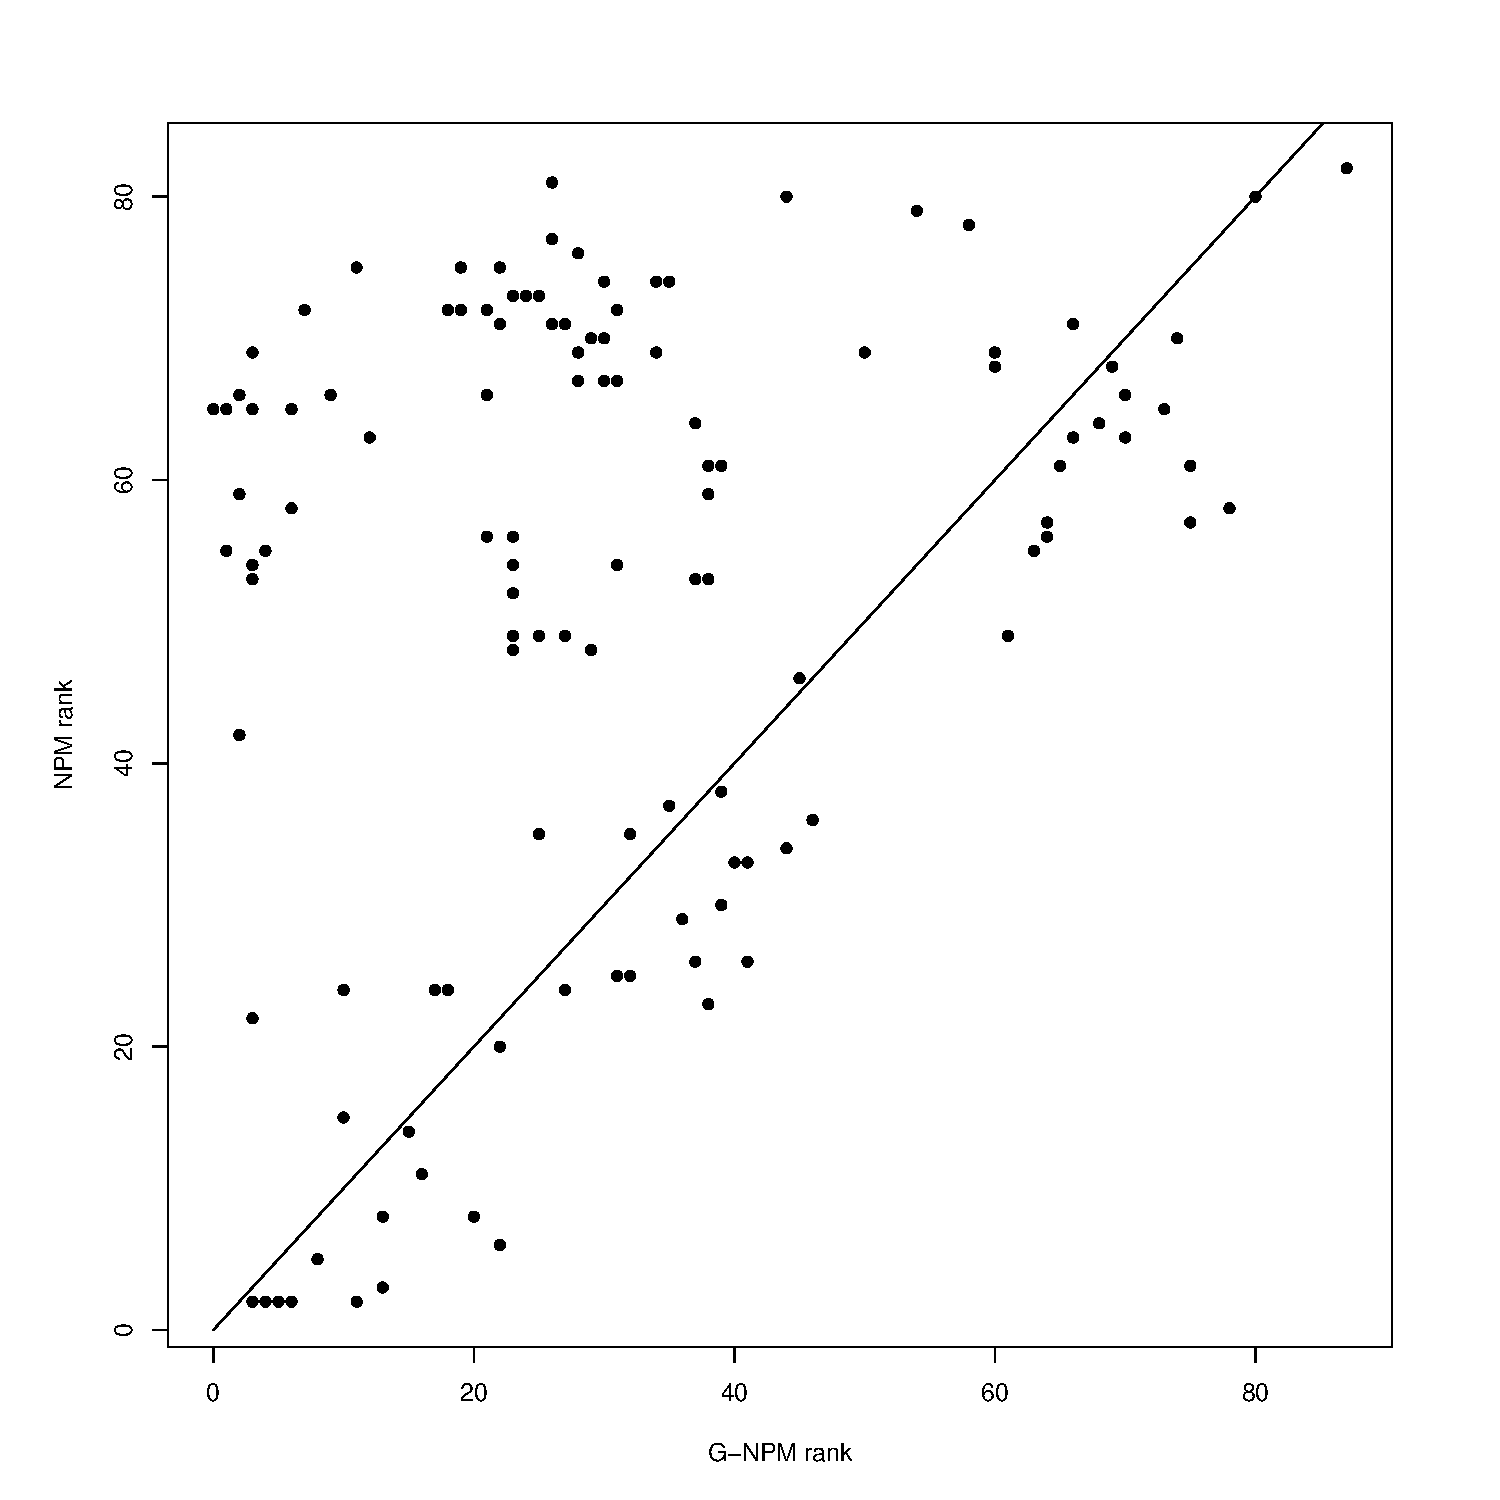
\includegraphics[width= 0.7\textwidth]{rq1.pdf}
\caption{Ranking Result of \name and \npm \label{fig:rq1}}
\end{figure}

Figure~\ref{fig:rq1} shows the ranking results visually. The X-axis is the ranking of relevant papers from \name and the Y-axis is the ranking of relevant papers from \npm. Clearly, the upper left part of the graphs shows the improvements of \name over \npm and the lower right area represents the negative cases which \name ranks worse than \npm. he number of positive cases is more than twice the number of negative cases. There were 248 positive cases and 107 negative cases. Furthermore, The ranking changes of positive cases were much greater than the ranking changes of negative cases. It means, in most of the cases, human effort to find relevant paper decreases dramatically, with little probability of small increase.

\begin{figure}[ht]
\centering
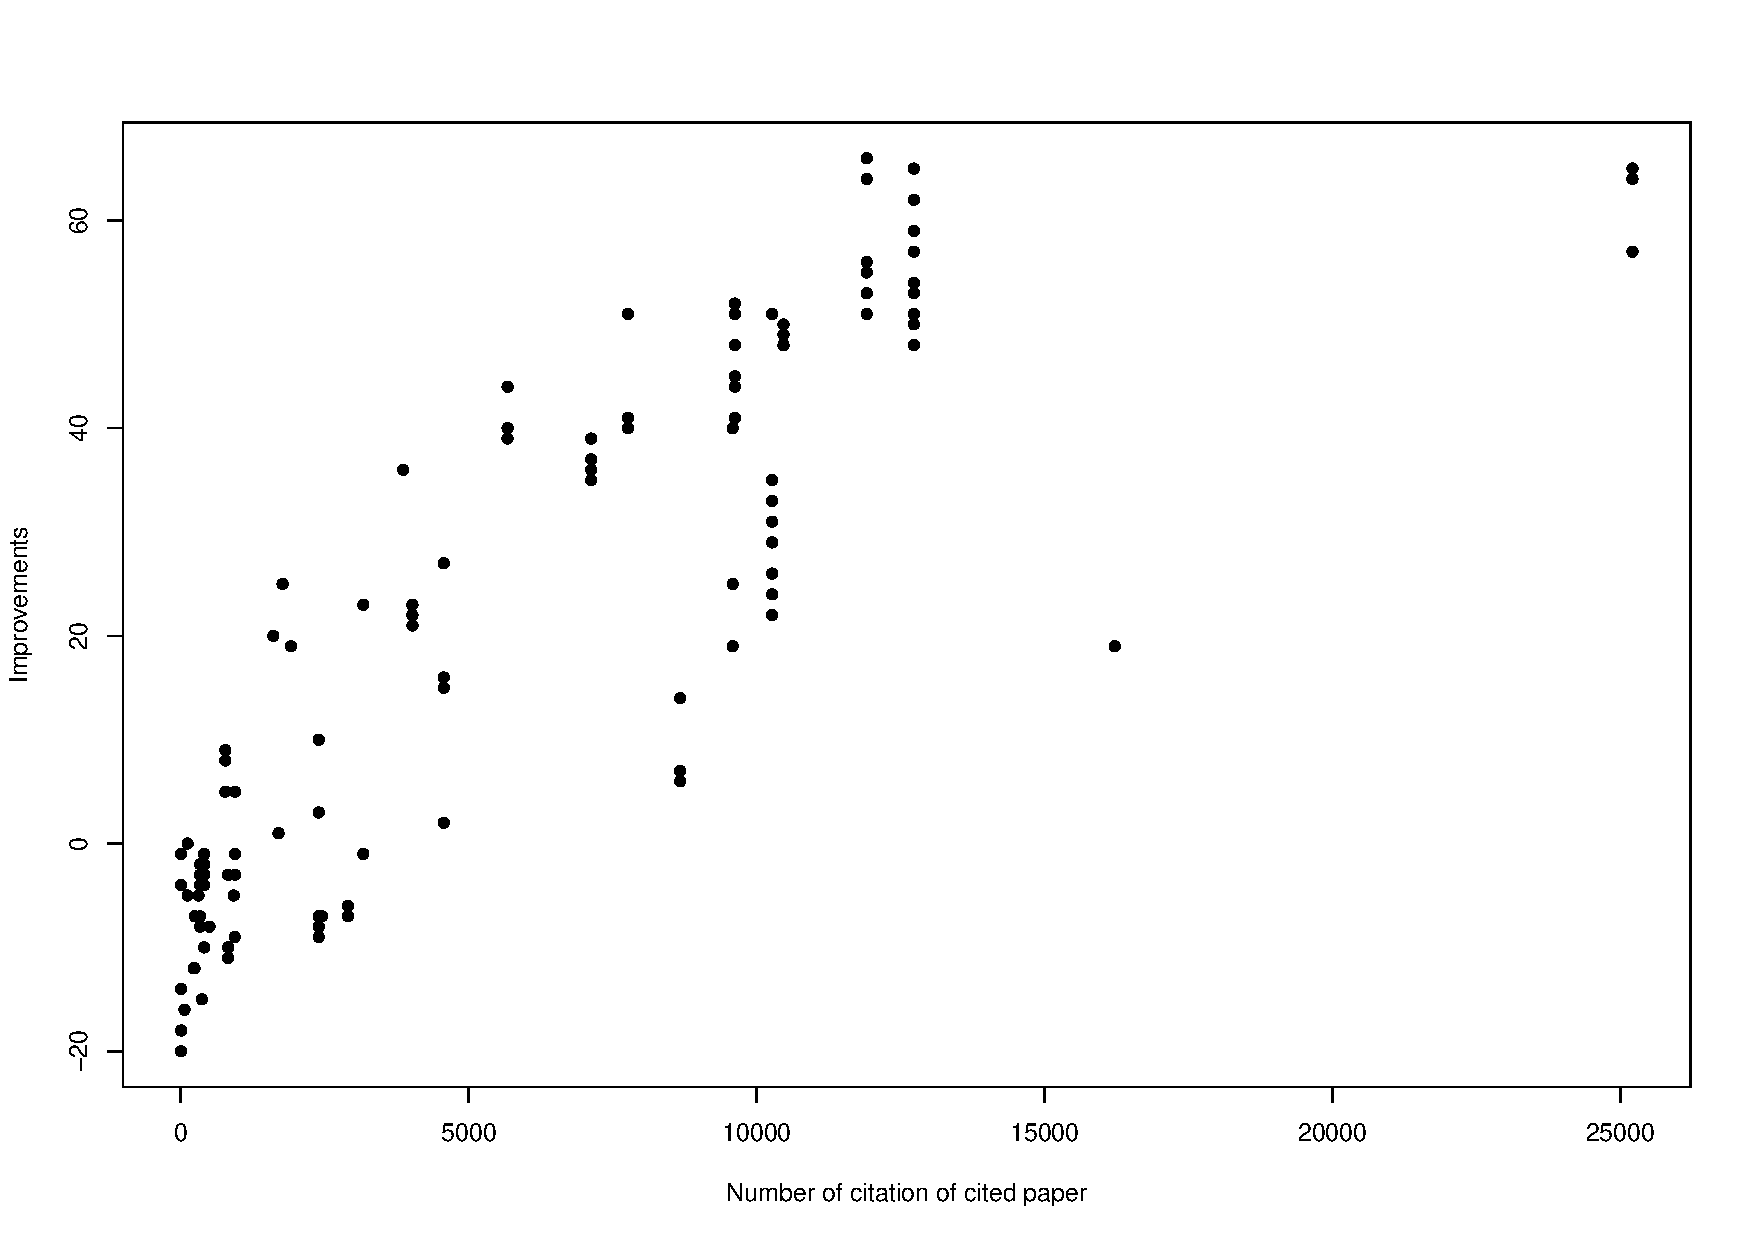
\includegraphics[width= \textwidth]{rq1_2.pdf}
\caption{Relation between ranking Improvements and citition count \label{fig:rq1_2}}
\end{figure}

Reminding motivation of the research, We tried to improve the ranking of highly cited paper. Figure~\ref{fig:rq1_2} shows that as the paper cited more, the improvement in ranking was greater.  The observation results about number of positive cases and negative cases and their effect size from Figure~\ref{fig:rq1}  can be re-observed in  Figure~\ref{fig:rq1_2}.


\subsection{Performance on Small Data Set}

In the experiments, We used small size of training data. Using small training data, the ranking results of \npm shows worse than \npm's original paper\cite{Huang:2015:NPM:2886521.2886655}. In the experiments, in spite of the use of small input data, the technique of \name model improved the results. \name can compensate for the poor results  of \npm from lack of training data.


\section{Discussion}


\subsection{Future works}

\begin{itemize}
\item Experiments of \name over large-scale training data set.\\
We could not evaluate the model in large data due to lack of computing power.
It is worth to confirm the performance of \name in a big data.\\

\item Add more global features such as venue or h-index.\\
In \name implementation, The number of citation of cited paper was only used as global feature. The global features from paper~\cite{Bethard:2010:ICL:1871437.1871517} could be the candidates. These includes venue, h-index, and etc.\\

\item Finding Novel formula combining NPM and global features\\
In \name implementation, We used simple weighted sum of \npm results and global features as scoring formula. Figure~\ref{fig:rq1_2} implies that the ranking improvements depends on the number of citation of cited paper. However simple weighted sum ignore the relation. Therefore, finding novel formula to combining two scores is desirable. Several machine-learning based approaches can be used to build the formula.
\end{itemize}


\subsection{Threats to Validity}

\begin{itemize}
\item Different retrieval date of citation count\\
In the usage of \name, The author considers the citation count of cited paper at the time of writing. Not only we were impossible to get a citation count at the time of writing, But also the whole data size grows rapidly if we considers the citation count at the time of writing.  For example, we need a vector $[\text{doc-id}, \text{count}_{19990130}, \text{count}_{19990314}, \dots, \text{count}_{20170521}, \text{count}_{20170615}]$ for each documents in data set.

Instead, we just used simple approach that uses only one citation count value at fixed date. There exists a difference between the citation count retrieval dates. Considering the highly-cited paper are likely to highly-cited further, there is a strong relationship between citation count at the time of writing and fixed point. This simple approximates able to approximate the citation count still effectively while saving the data size a lot.\\

\item Inaccurate citation count\\
We used a citation count which is captured by google scholar. So wrong results of Google scholar can pollute the citation count. To remove the pollution effect, we suggests to conduct experiments on a well structured citation count records for future works, such as database from \texttt{ACM}, or \texttt{IEEE}.
\end{itemize}



\section{Conclusion}
\label{sec:Conclusion}

In this paper we suggests adding global features to enhance the performance of local citation recommendation. We made \name prototype which uses citation count as global features. \name combines citation count information with original \npm. In our experiments, \name improved the ranking performance as double. \name competently shows performance improvements even in small size data. In further observation, \name shows greatly improvements on highly-cited papers, which were the weak point of the original \npm.

With little probability of small pain, we expect great probability of large gain from \name.



\bibliographystyle{splncs03}
\bibliography{ref}

\end{document}
